\documentclass[a4paper, 11pt]{article}

\usepackage[danish]{babel}
\usepackage[utf8]{inputenc}
%\usepackage{tgtermes}
%\usepackage{fouriernc}
\usepackage[T1]{fontenc}
\usepackage[margin=3cm]{geometry}

\usepackage{graphicx}
\usepackage{amssymb}
\usepackage{amsmath}
\usepackage{amsthm}
\usepackage{multicol}
\usepackage{xcolor}
\usepackage{wrapfig}

\usepackage{enumerate}
\usepackage[shortlabels]{enumitem}
\usepackage{verbatim}
\usepackage{hyperref}
\hypersetup{
    colorlinks=true,
    linkcolor=red,   
    urlcolor=red,
}
\newcommand{\N}{\mathbb{N}}
\newcommand{\Z}{\mathbb{Z}}
\newcommand{\Q}{\mathbb{Q}}
\newcommand{\R}{\mathbb{R}}

%Is defined to be equal to
\newcommand*{\defeq}{\mathrel{\vcenter{\baselineskip0.5ex \lineskiplimit0pt
                     \hbox{\scriptsize.}\hbox{\scriptsize.}}}%
                     =}
 
\title{{\large \textsc{Projekt Blodsukker}}}
\author{Cecilie Horshauge}
\date{\today}

\begin{document}
\maketitle
% Intro til opgaven
\noindent Hos raske mennesker reguleres blodsukkerkoncentrationen automatisk via leveren. 
Normalt ligger koncentrationen i intervallet 60-100 mg blodsukker pr. 100 ml blod. 
Hormonet insulin har den virkning, at det stimulerer cellernes optagelse af sukker fra blodet. 
Det følgende drejer sig om en forsøgsperson, der får en indsprøjtning af en bestemt dosis insulin.\\\\
Efter indsprøjtningen vil blodsukkerkoncentrationen ændre sig som funktion af den tid,
der er forløbet efter indsprøjtningen. Det antages i det følgende, at denne funktion med god tilnærmelse kan beskrives på følgende form: 
\[C(t)=83+75\cdot (a^t-b^t) \;\;\; \text{mg pr. 100 mL}\]
hvor \(t\) er målt i timer og \(a=0.1\), \(b=0.5\)

\section*{Opgave A} 
Beskriv med ord hvorledes koncentrationen udvikler sig på kort, lidt længere og på helt langt sigt.

\subsection*{Løsning}
Ved \(t=0\), funktionens "begyndelse", vil koncentrationen have værdien \(83\) mg pr. 100 mL. Som \(t\) langsomt stiger vil koncentrationen til at begynde med falde hurtigt. På et tidspunkt vil udviklingen stoppe med at falde. Man kan sammenligne \(t=1\) og \(t=2\). Her får vi følgende:
\begin{align*}
    C(1)&=83+75 \cdot (0.1^1-0.5^1)=83+75 \cdot (-0.4)\\
    C(2)&=83+75 \cdot (0.1^2-0.5^2)=83+75 \cdot (-0.24)
\end{align*} 
Her bliver det altså klart at inden 2 timer er gået vil koncentrationen begynde at stige igen. Som \(t\) fortsat stiger vil forskellen mellem de to kvadrater blive mindre og mindre og koncentrationen vil gå mod 83 mg pr. 100 mL igen.
\clearpage
\section*{Opgave B} 
Hvad er den laveste koncentration, som forsøgspersonen oplever?
\subsection*{Løsning}
Først bestemmes \(c'(t)\).\\
\begin{align*}
    c'(t)&=(83+75 \cdot (a^t-b^t))'\\
    &= (83)'+ 75 \cdot ((a^t)'-(b^t)')\\
    &= 0+ 75 \cdot (a^t\cdot \ln(a)-b^t\cdot \ln(b))\\
\end{align*}
Nu vil vi isolere \(t\) i ligningen \(c'(t)=0\).
\begin{align*}
    0 &= 75 \cdot (a^t\cdot \ln(a)-b^t\cdot \ln(b))\\
    0 &= a^t\cdot \ln(a)-b^t\cdot \ln(b)\\
    b^t \cdot \ln(b) &= a^t\cdot \ln(a)\\
    \frac{\ln(b)}{\ln(a)}&=\frac{a^t}{b^t}\\
    \frac{\ln(b)}{\ln(a)}&=\left(\frac{a}{b}\right)^t\\
    \ln\left(\frac{\ln(b)}{\ln(a)}\right) &= \ln\left(\left(\frac{a}{b}\right)^t \right)\\
    \ln(\ln(b))-\ln(\ln(a)) &= t\cdot (\ln(a)-\ln(b))\\\\
    t &= \frac{\ln(\ln(b))-\ln(\ln(a))}{\ln(a)-\ln(b)}
    \intertext{Vi indsætter \(a\) og \(b\) og bestemmer \(t\)}
    t &= \frac{\ln(\ln(0.5))-\ln(\ln(0.1))}{\ln(0.1)-\ln(0.5)}=\textcolor{blue}{0.7459407766}
\end{align*}
Nu da \(t\) er bestemt kan vi indsætte det fundne \(t\) i funktionen og bestemme koncentrationen.\\
\(c(0.7459407766)=\textcolor{blue}{51.74141941}\)

\subsection*{Løsning med CAS}
\(a \defeq 0.1\, \colon\, b \defeq 0.5 \, \colon\)\\
\(c\left(t\right)\defeq 83+75\cdot \left(a^{t}-b^{t}\right)\colon\)\\
\(t_{\mathit{lav}}\defeq \mathit{solve}\left(c'\left(t\right)=0\right)=\textcolor{blue}{0.7459407764}\)\\
\(c(t_{lav})=\textcolor{blue}{51.74141940}\)\\\\
\textbf{Den laveste koncentration, som forsøgspersonen oplever, er 51.74 mg pr. 100 mL.}
\clearpage
\section*{Opgave C} 
Hvornår falder koncentrationen hurtigst og hvornår stiger den hurtigst?
\subsection*{Løsning}
Det største fald og den største stigning hos en funktion kan altid findes ved ekstremum, der i nogle tilfælde kan findes ved endepunkterne af funktionens afledte funktion.\\
Betragt først grafen for \(c'(t)\).\\
\begin{center}
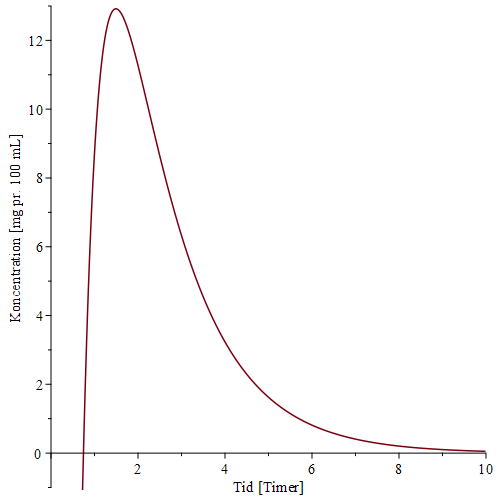
\includegraphics[width = 0.65 \textwidth]{AfledtGraf.png}
\end{center}
Her bemærker vi et maksimum mellem 1 og 2 og at minimum der ser ud til at ligge i 0. Det er let at bestemme maksimum, vi kan blot benytte et CAS-værktøj til at isolere \(t\) i ligningen \(c''(t)=0\).\\
\(\mathit{solve}\left(c''\left(t\right)=0\right)=\textcolor{blue}{1.491881553}\)\\
Lad os nu overbevise os selv om at minimum hos den afledte funktion kan findes ved \(t=0\). 
\[c'(t)=- 172.6938820 \cdot 0.1^{t}+ 51.98603854 \cdot 0.5^{t}\]
Som \(t\) nærmer sig \(0\) vil både \(0.1^t\) og \(0.5^t\) nærme sig \(1\). Dog nærmer \(0.5^t\) siger hurtigere. Første led er mest negativt når \(t=0\), og det bliver gradvist mere negativt som \(t\) nærmer sig 0. På samme måde bliver andet led også større som \(t\) går mod 0. Leddet kan dog ikke blive større end ca. 52, hvor første led bliver betydeligt mere negativt som \(t\) nærmer sig 0. Det giver derfor også mening at mimimum må ligge i \(t=0\).\\\\
\textbf{Koncentrationen falder altså hurtigst ved \(t=0\) og stiger hurtigst ved \(t=1.49\).}
\clearpage
\section*{Opgave D} 
Hvornår vil funktionsværdien være inden for l\% fra sin asymptotiske værdi?
\subsection*{Løsning}
Den asymptotiske værdi er 83, som tidligere nævnt vil koncentrationen netop gå mod 83 som \(t\) bliver større. 
Men på intet tidspunkt bliver koncentrationen større end 83 mg pr. 100 mL. Derfor bestemmer jeg den nedre grænse for 1\% rækkevidde.\\ 
\(83 \cdot 0.99 = \textcolor{blue}{82.17}\)\\
Der må være 2 steder hvor koncentrationen er indenfor 1\% af den asymptotiske værdi, en gang tidligt og en gang sent. De bestemmes ved\\
\(solve(82.17=c(t))\)
\[\textcolor{blue}{0.006948004966}\]
\(\mathit{fsolve}\left(83\cdot  0.99=c\left(t\right),t=6\right)\)
\[\textcolor{blue}{6.497593996}\]
\textbf{Funktionen er inden for 1\% af sin asymptotiske værdi indtil \(t=0.007\) og efter \(t=0.6.498\).}
\section*{Opgave E} 
Man kan føle et stærkt ubehag, hvis blodsukkerkoncentrationen falder til under 60 mg pr. 100 ml. \\
I hvilket tidsrum efter indsprøjtningen må forsøgspersonen være forberedt på ubehag?
\subsection*{Løsning}
Vi leder efter 2 tidspunkter hvor modellen har koncentrationen 60 mg pr. 100 mL. \\
\(solve(60 = c(t),t)\)
\[\textcolor{blue}{ 1.588835746, 0.2926616696}\]
\textbf{Altså vil man føle et stærkt ubehag mellem 0.293 og 1.589 timer efter indsprøjtningen.}
\end{document}